\usetikzlibrary{calc}
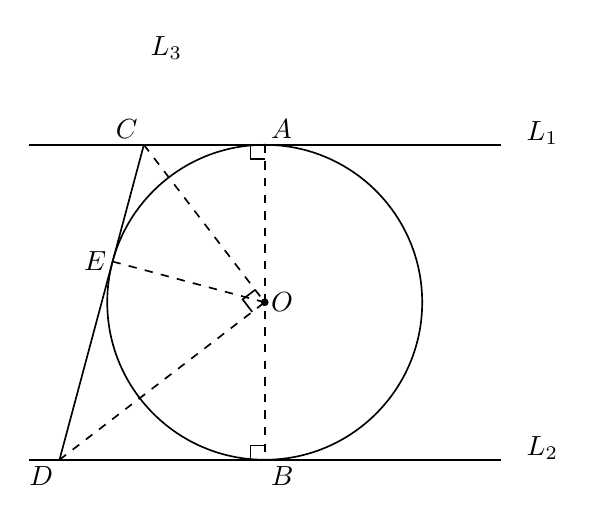
\begin{tikzpicture}[x=1cm,y=1cm,line width=.6pt,font=\normalsize]
\coordinate (O) at (0,0);
\coordinate (A) at (0,2);
\coordinate (B) at (0,-2);
\coordinate (E) at (-1.9319,0.5176);
\coordinate (C) at (-1.5347,2);
\coordinate (D) at (-2.6065,-2);
\draw (O) circle[radius=2cm];
\draw (C)--(3,2);
\draw (-3,2)--(C);
\draw (D)--(3,-2);
\draw (-3,-2)--(D);
\draw (C)--(D);
\draw[dashed] (A)--(B);
\draw[dashed] (E)--(O);
\draw[dashed] (C)--(O);
\draw[dashed] (D)--(O);
\node[above right=2pt,inner sep=0pt] at (A) {$A$};
\node[below right=2pt,inner sep=0pt] at (B) {$B$};
\node[above left=2pt,inner sep=0pt] at (C) {$C$};
\node[below left=2pt,inner sep=0pt] at (D) {$D$};
\node[left=2pt,inner sep=0pt] at (E) {$E$};
\node[right=2pt,inner sep=0pt] at (O) {$O$};
\node[right] at (3.2,2.15) {$L_{1}$};
\node[right] at (3.2,-1.85) {$L_{2}$};
\node[above] at (-1.25,2.95) {$L_{3}$};
\draw (-.18,2)--(-.18,1.82)--(0,1.82);
\draw (-.18,-2)--(-.18,-1.82)--(0,-1.82);
\draw (-.1218,.1586)--(-.2804,.0368)--(-.1586,-.1218);

% Explicit named circle-center points, painted after all region fills.
\fill (O) circle[radius=1.4pt];
\end{tikzpicture}
